%%%%%%%%%%%%%%%%%%%%%%%%%%%%%%%%%%%%%%%%%
% Lachaise Assignment
% LaTeX Template
% Version 1.0 (26/6/2018)
%
% This template originates from:
% http://www.LaTeXTemplates.com
%
% Authors:
% Marion Lachaise & François Févotte
% Vel (vel@LaTeXTemplates.com)
%
% License:
% CC BY-NC-SA 3.0 (http://creativecommons.org/licenses/by-nc-sa/3.0/)
% 
%%%%%%%%%%%%%%%%%%%%%%%%%%%%%%%%%%%%%%%%%

%----------------------------------------------------------------------------------------
%	PACKAGES AND OTHER DOCUMENT CONFIGURATIONS
%----------------------------------------------------------------------------------------

\documentclass{article}

%%%%%%%%%%%%%%%%%%%%%%%%%%%%%%%%%%%%%%%%%
% Lachaise Assignment
% Structure Specification File
% Version 1.0 (26/6/2018)
%
% This template originates from:
% http://www.LaTeXTemplates.com
%
% Authors:
% Marion Lachaise & François Févotte
% Vel (vel@LaTeXTemplates.com)
%
% License:
% CC BY-NC-SA 3.0 (http://creativecommons.org/licenses/by-nc-sa/3.0/)
% 
%%%%%%%%%%%%%%%%%%%%%%%%%%%%%%%%%%%%%%%%%

%----------------------------------------------------------------------------------------
%	PACKAGES AND OTHER DOCUMENT CONFIGURATIONS
%----------------------------------------------------------------------------------------

\usepackage{amsmath,amsfonts,stmaryrd,amssymb} % Math packages

\usepackage{enumerate} % Custom item numbers for enumerations

\usepackage[ruled]{algorithm2e} % Algorithms

\usepackage[framemethod=tikz]{mdframed} % Allows defining custom boxed/framed environments

\usepackage{listings} % File listings, with syntax highlighting
\lstset{
	basicstyle=\ttfamily, % Typeset listings in monospace font
}

%----------------------------------------------------------------------------------------
%	DOCUMENT MARGINS
%----------------------------------------------------------------------------------------

\usepackage{geometry} % Required for adjusting page dimensions and margins

\geometry{
	paper=a4paper, % Paper size, change to letterpaper for US letter size
	top=2.5cm, % Top margin
	bottom=3cm, % Bottom margin
	left=2.5cm, % Left margin
	right=2.5cm, % Right margin
	headheight=14pt, % Header height
	footskip=1.5cm, % Space from the bottom margin to the baseline of the footer
	headsep=1.2cm, % Space from the top margin to the baseline of the header
	%showframe, % Uncomment to show how the type block is set on the page
}

%----------------------------------------------------------------------------------------
%	FONTS
%----------------------------------------------------------------------------------------

\usepackage[utf8]{inputenc} % Required for inputting international characters
\usepackage[T1]{fontenc} % Output font encoding for international characters

\usepackage{XCharter} % Use the XCharter fonts

%----------------------------------------------------------------------------------------
%	COMMAND LINE ENVIRONMENT
%----------------------------------------------------------------------------------------

% Usage:
% \begin{commandline}
%	\begin{verbatim}
%		$ ls
%		
%		Applications	Desktop	...
%	\end{verbatim}
% \end{commandline}

\mdfdefinestyle{commandline}{
	leftmargin=10pt,
	rightmargin=10pt,
	innerleftmargin=15pt,
	middlelinecolor=black!50!white,
	middlelinewidth=2pt,
	frametitlerule=false,
	backgroundcolor=black!5!white,
	frametitle={Command Line},
	frametitlefont={\normalfont\sffamily\color{white}\hspace{-1em}},
	frametitlebackgroundcolor=black!50!white,
	nobreak,
}

% Define a custom environment for command-line snapshots
\newenvironment{commandline}{
	\medskip
	\begin{mdframed}[style=commandline]
}{
	\end{mdframed}
	\medskip
}

%----------------------------------------------------------------------------------------
%	FILE CONTENTS ENVIRONMENT
%----------------------------------------------------------------------------------------

% Usage:
% \begin{file}[optional filename, defaults to "File"]
%	File contents, for example, with a listings environment
% \end{file}

\mdfdefinestyle{file}{
	innertopmargin=1.6\baselineskip,
	innerbottommargin=0.8\baselineskip,
	topline=false, bottomline=false,
	leftline=false, rightline=false,
	leftmargin=2cm,
	rightmargin=2cm,
	singleextra={%
		\draw[fill=black!10!white](P)++(0,-1.2em)rectangle(P-|O);
		\node[anchor=north west]
		at(P-|O){\ttfamily\mdfilename};
		%
		\def\l{3em}
		\draw(O-|P)++(-\l,0)--++(\l,\l)--(P)--(P-|O)--(O)--cycle;
		\draw(O-|P)++(-\l,0)--++(0,\l)--++(\l,0);
	},
	nobreak,
}

% Define a custom environment for file contents
\newenvironment{file}[1][File]{ % Set the default filename to "File"
	\medskip
	\newcommand{\mdfilename}{#1}
	\begin{mdframed}[style=file]
}{
	\end{mdframed}
	\medskip
}

%----------------------------------------------------------------------------------------
%	NUMBERED QUESTIONS ENVIRONMENT
%----------------------------------------------------------------------------------------

% Usage:
% \begin{question}[optional title]
%	Question contents
% \end{question}

\mdfdefinestyle{question}{
	innertopmargin=1.2\baselineskip,
	innerbottommargin=0.8\baselineskip,
	roundcorner=5pt,
	nobreak,
	singleextra={%
		\draw(P-|O)node[xshift=1em,anchor=west,fill=white,draw,rounded corners=5pt]{%
		Question \theQuestion\questionTitle};
	},
}

\newcounter{Question} % Stores the current question number that gets iterated with each new question

% Define a custom environment for numbered questions
\newenvironment{question}[1][\unskip]{
	\bigskip
	\stepcounter{Question}
	\newcommand{\questionTitle}{~#1}
	\begin{mdframed}[style=question]
}{
	\end{mdframed}
	\medskip
}

%----------------------------------------------------------------------------------------
%	WARNING TEXT ENVIRONMENT
%----------------------------------------------------------------------------------------

% Usage:
% \begin{warn}[optional title, defaults to "Warning:"]
%	Contents
% \end{warn}

\mdfdefinestyle{warning}{
	topline=false, bottomline=false,
	leftline=false, rightline=false,
	nobreak,
	singleextra={%
		\draw(P-|O)++(-0.5em,0)node(tmp1){};
		\draw(P-|O)++(0.5em,0)node(tmp2){};
		\fill[black,rotate around={45:(P-|O)}](tmp1)rectangle(tmp2);
		\node at(P-|O){\color{white}\scriptsize\bf !};
		\draw[very thick](P-|O)++(0,-1em)--(O);%--(O-|P);
	}
}

% Define a custom environment for warning text
\newenvironment{warn}[1][Warning:]{ % Set the default warning to "Warning:"
	\medskip
	\begin{mdframed}[style=warning]
		\noindent{\textbf{#1}}
}{
	\end{mdframed}
}

%----------------------------------------------------------------------------------------
%	INFORMATION ENVIRONMENT
%----------------------------------------------------------------------------------------

% Usage:
% \begin{info}[optional title, defaults to "Info:"]
% 	contents
% 	\end{info}

\mdfdefinestyle{info}{%
	topline=false, bottomline=false,
	leftline=false, rightline=false,
	nobreak,
	singleextra={%
		\fill[black](P-|O)circle[radius=0.4em];
		\node at(P-|O){\color{white}\scriptsize\bf i};
		\draw[very thick](P-|O)++(0,-0.8em)--(O);%--(O-|P);
	}
}

% Define a custom environment for information
\newenvironment{info}[1][Info:]{ % Set the default title to "Info:"
	\medskip
	\begin{mdframed}[style=info]
		\noindent{\textbf{#1}}
}{
	\end{mdframed}
}
 % Include the file specifying the document structure and custom commands

\usepackage{hyperref}

\usepackage{siunitx}

%----------------------------------------------------------------------------------------
%	ASSIGNMENT INFORMATION
%----------------------------------------------------------------------------------------

\title{LO block VCO and VCO Buffer} % Title of the assignment

\author{Aleksandar Vuković} % Author name and email address

\date{\today} % University, school and/or department name(s) and a date

%----------------------------------------------------------------------------------------

\begin{document}

\maketitle % Print the title

%----------------------------------------------------------------------------------------
%	INTRODUCTION
%----------------------------------------------------------------------------------------

\section*{Introduction} % Unnumbered section

LO block is LC VCO with internal inductor and fully differential output buffer. Its schematic shall ensure differential connection to the mixer LO input and PLL RF input. LO block should have the characteristics given in Table \ref{table-spec}. Due to wide frequency range it is necessary to use switchable capacitor banks.  

%----------------------------------------------------------------------------------------
\section{Technical Requirements}


\begin{table}[ht]
	\centering
	\begin{tabular}{|c|l|c|c|c|c|c|}
		\hline
		& LO Requirements & Note & min & typ & max & Units \\
		\hline
		& \multicolumn{6}{|c|}{VCO Requirements} \\
		\hline
		1 & Full LO range &  & 6300  &  & 13700 & MHz \\ 
		\hline
		2 & Phase Noise at 300 kHz &  &  &  & <-101 & dBc/Hz \\ 
		\hline
		3 & Vtune &  & 0.1 &  & 1 & V  \\ 
		\hline
		4 & Tuning Sensitivity $K_{VCO}$ &  &  &  & 100 & MHz/V  \\ 
		\hline
		5 & Pushing & TBD &  &  & 2 & MHz/V  \\ 
		\hline
		6 & Output Voltage & TBD & 0.8 &  & & $V_{p-p}$  \\ 
		\hline
		7 & Load Impedance &  &  &  & 100 & fF  \\ 
		\hline
		& \multicolumn{6}{|c|}{VCO and output Buffer} \\
		\hline
		8 & Output Voltage & TBD & 0.8  &  &  & V  \\ 
		\hline
		9 & Load Impedance & TBD &  &  & 1000 & fF  \\ 
		\hline
		10 & Harmonic suppression ($2_{nd}$, typ) &  & -15 &  &  & dBc  \\ 
		\hline
		11 & Pulling (14 dB Return Loss, Any Phase) & TBD &  &  & 2 & MHz  \\ 
		\hline
		& \multicolumn{6}{|c|}{General Specifications} \\
		\hline
		12 & Operating Temperature Range &  & -40 &  & 125 & °C  \\ 
		\hline
		13 & Supply Voltage &  & 1 & 1.1 & 1.2 & V  \\ 
		\hline
		14 & Supply Current &  &  &  & 20 & mA  \\ 
		\hline
		15 & Shutdown Current &  &  &  & 10 & $\mu$A  \\ 
		\hline
		16 & Time to Switch Between Cores  &  &  & 3 & 5 & ms  \\ 
		\hline
	\end{tabular}
	\label{table-spec}
	\caption{Specification Requirements} 

\end{table}

Min and max for supply voltage are not defined in the original document, and time for switching between two cores was defined during the meeting.

Currently Full LO range is split between two cores so the requirement should look like this:

\begin{table}[ht]
	\centering
	\begin{tabular}{|c|l|c|c|c|c|c|}
		\hline
		& LO range requirements & Note & min & typ & max & Units \\
		\hline
		1 & High Band core LO range &  & 10000  &  & 13700 & MHz \\ 
		\hline
		2 & Low Band core LO range &  & 6300 &  & 10000 & MHz \\ 
		\hline
	\end{tabular}
	\caption{LO Range Two Core Specification Requirements} 
\end{table}

\begin{question}[\itshape What's the variation for supply voltage?]
	Not defined probably will be the same as the rest of the 
\end{question}


\begin{question}[\itshape $K_{VCO}$ Why is it in the max column? ]
	Didn't get answer for this. It's probably also typical and a value that is expected by the PLL design.
\end{question}

% Footnotes do not work.

Process corners can be found at:

\begin{verbatim}
/tech/tsmc/tsmc40/models/spectre/crn40lp_2d5_v2d0_2_shrink0d9_embedded_usage.scs
\end{verbatim}
% Seems that 

\section{Scaldio Design Review}

\begin{question}[\itshape How should calibration be implemented to achieve output voltage peak to peak and minimize noise?]
Is it done for whole PLL?
\end{question}

\begin{question}[\itshape Difference between class-B and class-C vco? ]
	Scaldio uses class-C, so all parasitic capacitances connected to the tail don't matter. Having trouble with observing the currents of drain so cannot check this and compare them. Scaldio looks something between class C and class B because of $V_{gbias}$ voltage and because adding inductor between tail NMOS and switching pair improves phase noise. This is attributed to class B, while class C only needs tail capacitance.
\end{question}




% \begin{figure}[ht!]
% 	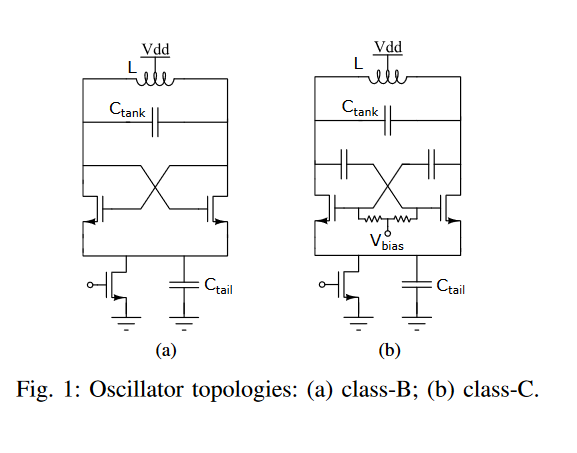
\includegraphics[width=\linewidth]{Figures/class_C_vs_class_B.png}
% 	% \caption{Difference between class C and class B}
% 	\label{fig:classC_classB}
% \end{figure}

\begin{figure}[ht!]
	\centering
	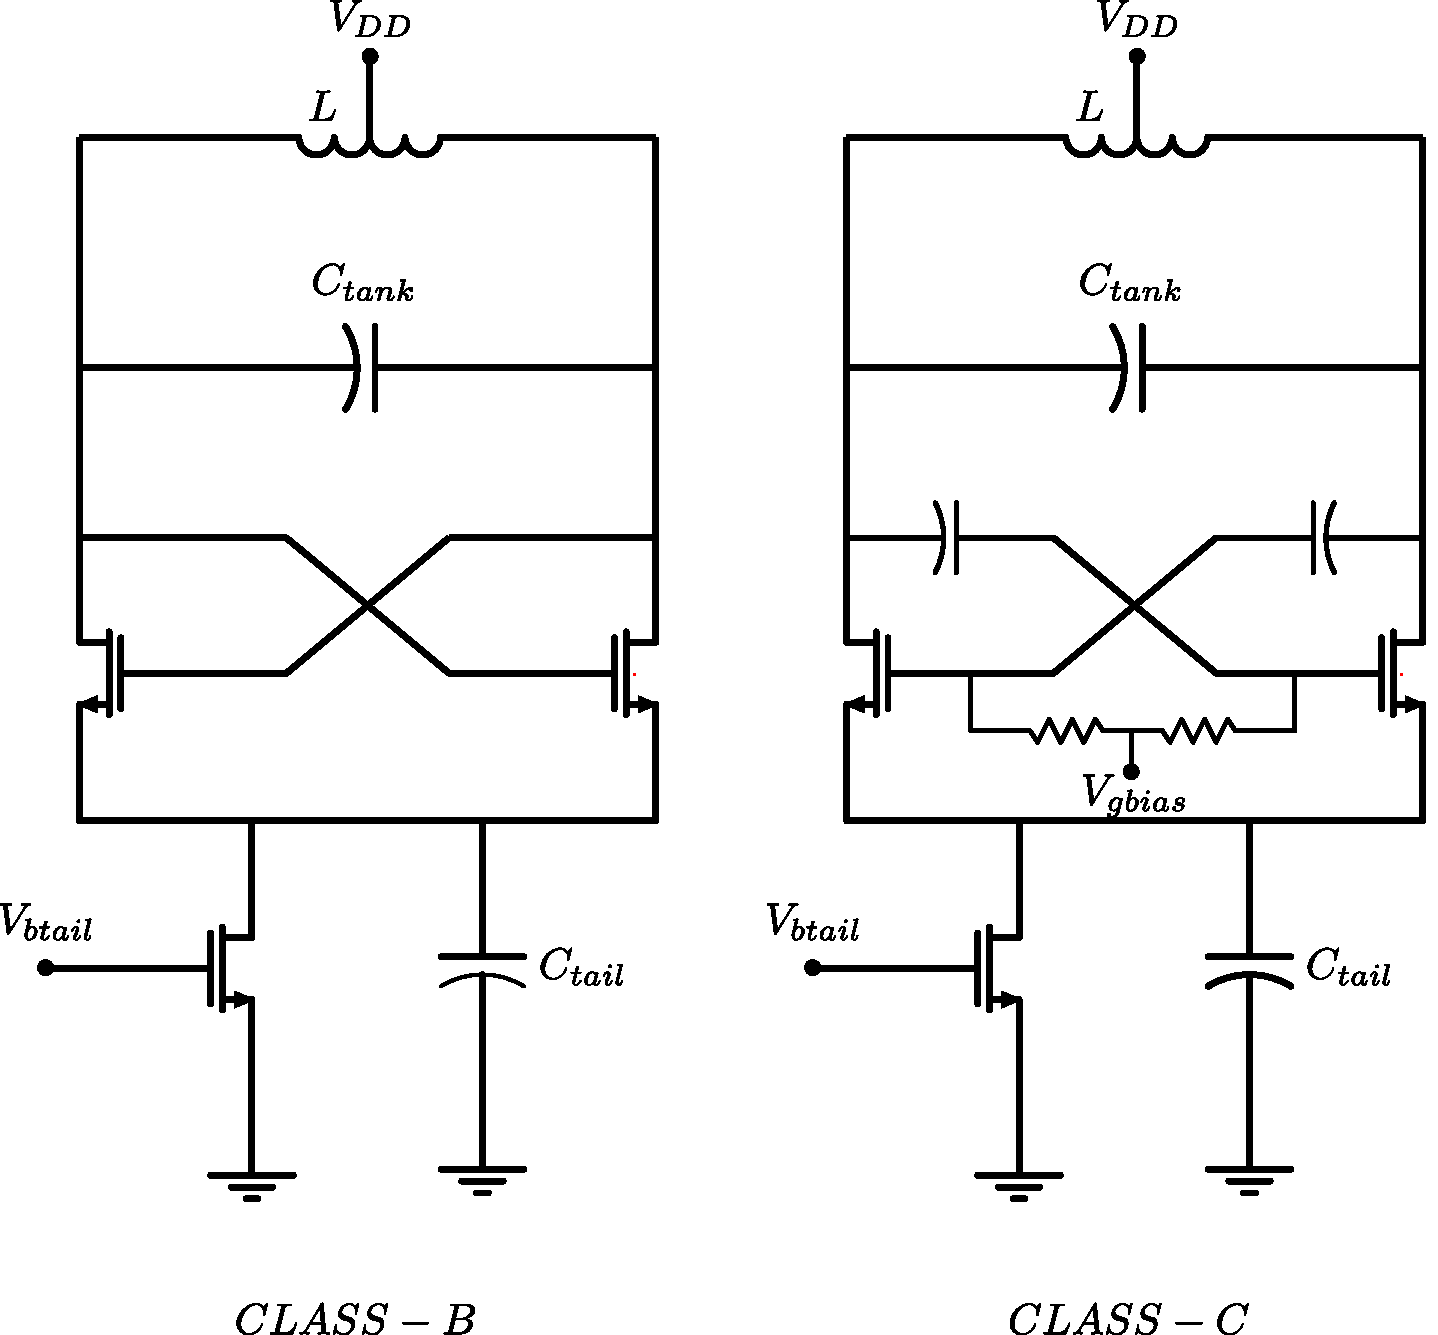
\includegraphics[width=0.7\linewidth]{Figures/class-B_vs_class-C.pdf}
	\caption{Schematic difference between class C and class B}
	\label{fig:classC_classB_inkscape}
\end{figure}


Lowest bit of digital varactor (L0\_PLL\_hbVCO\_Cdig\_SC2B\_VCOS\_SC2C\_PLL) doesn't do anything, isn't even monotonous. Maybe makes more sense when simulating extracted cells. Digital varactor needs to be redesigned, it could lower the Q factor.
Main difference between class B and class C can be observed by investigating their drain currents.

\begin{figure}[ht!]
	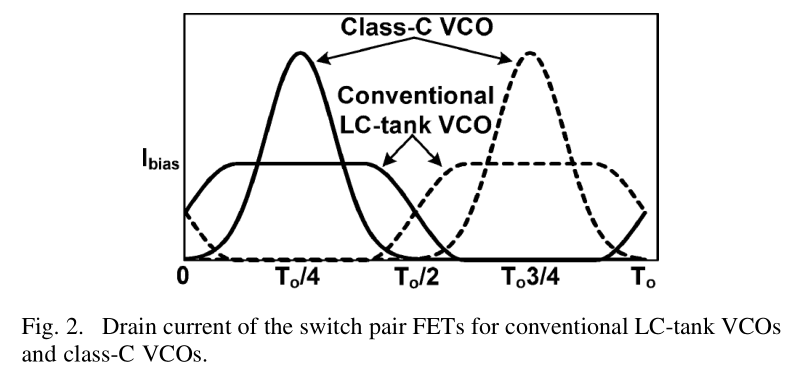
\includegraphics[width=\linewidth]{Figures/drainCurrent_classB_vs_classC.png}
	% \caption{Difference between class C and class B}
	\label{fig:drainCurrent_classB_vs_classC}
\end{figure}

\subsection{Main testbench}

Main testbench covers everything except for frequency pulling and full LO range. The simulation results are obtained at the higher end of the LO range. Phase noise is simulated by pss+pnoise.

\begin{info} % Information block
	With Noise Type=timeaverage and ALL(AM,PM,USB,LSB), you can plot the AM and PM components as well as the total noise. In addition, you can plot phase noise and FM jitter results for oscillators. Plotting is done using the Direct Plot Form.
	\href{https://community.cadence.com/cadence_blogs_8/b/rf/posts/virtuoso-video-diary-noise-simulation-in-spectre-rf-using-improved-pnoise-hbnoise-and-direct-plot-form-options}{\textbf{External link}}
\end{info}

Function of phase noise is simulated for PM noise type.

How to choose beat frequency for autonomous system from forum \href{https://community.cadence.com/cadence_technology_forums/f/custom-ic-design/2661/beat-frequency-in-spectrerf-pss-simulation}{\textbf{thread}}.

\begin{info} % Information block
In an autonomous system (e.g. an oscillator), you turn on the "oscillator" checkbox, and the beat frequency is then the estimated frequency, which gives PSS a starting point to solve for the oscillator frequency. It's important when in oscillator mode to select the outputs of the circuit, which include any subharmonics. In other words, if you have an oscillator followed by a divider, point at the divider output, and give the estimated divided frequency as the beat frequency. Again, this is because you need to solve an integer number of cycles of all the frequencies in the circuit. Note, don't use oscillator mode for circuits which aren't oscillators, since you're then trying to get the simulator to solve for an unknown which is not unknown, which may lead to convergence problems.
\end{info}

Most of the $I_{bias}$ tune digital control is not used for the higher band, so by increasing the number of steps to cover even higher frequencies than the original design finer bias control is needed.


\subsection{Simulation Results for Scaldio design}

Simulated only nominal corner with change for $V_{DD}$ only for frequency pushing simulation. 

\begin{table}[ht]
	\centering
	\begin{tabular}{|c|l|c|c|c|c|c|c|}
		\hline
		& LO Requirements & Note & min & typ & max & Sim(Typ) & Units \\
		% \hline
		% & \multicolumn{7}{|c|}{VCO Requirements} \\
		\hline
		1 & Phase Noise at 300 kHz &  &  &  & <-101 & -98 & dBc/Hz  \\ 
		\hline
		2 & Tuning Sensitivity $K_{VCO}$ &  &  &  & 100 & over & MHz/V  \\ 
		\hline
		3 & Pushing & TBD &  &  & 2  & 279.7 & MHz/V  \\ 
		\hline
		4 & Output Voltage & TBD & 800 &  & & 809.3 & $mV_{p-p}$  \\ 
		\hline
		5 & Harmonic suppression ($2_{nd}$, typ) &  & -15 &  & & -26.78 & dBc  \\ 
		\hline
		6 & Pulling (14 dB Return Loss, Any Phase) & TBD &  &  & 2  & 19.51 & MHz  \\ 
		\hline
	\end{tabular}
	\label{table-ScaldioResults}
	\caption{Scaldio IMEC design Results}
\end{table}

Phase noise changes a lot for different tuning voltages between -90 and -100 dBc/Hz. Phase noise is probably not modeled ok because the VCO doesn't have the connection between current bias tail and the switching pair of VCO as transmission line. That inductance and $C_{tail}$ should resonate at 2$\omega_O$ (tank oscillating frequency), but only in the case of class B oscillator. Check what type is vco oscillator. %This is hard to check because pss\_tran drain currents look wierd.

\newpage

%----------------------------------------------------------------------------------------
\section{Q factor of LC tank}

Need testbenches capacitance of tank, varactors and inductor, and for different controls and also corners. Process corners for varactors are the same as MOSFET.

% and of tail (to see how to make it resonate at the double of the oscillating frequency).

\begin{question}[\itshape What kind of chip is it?]
	What kind of inductance is expected to be connected on $V_{DD}$ and $V_{SS}$ pins. This may or may not change the results. Removed all together right now.
\end{question}

Testbench for differential Q and L of the inductor that is EMX simulated is shown in Figure \ref{fig:qlinductor}.

\begin{figure}[ht!]
	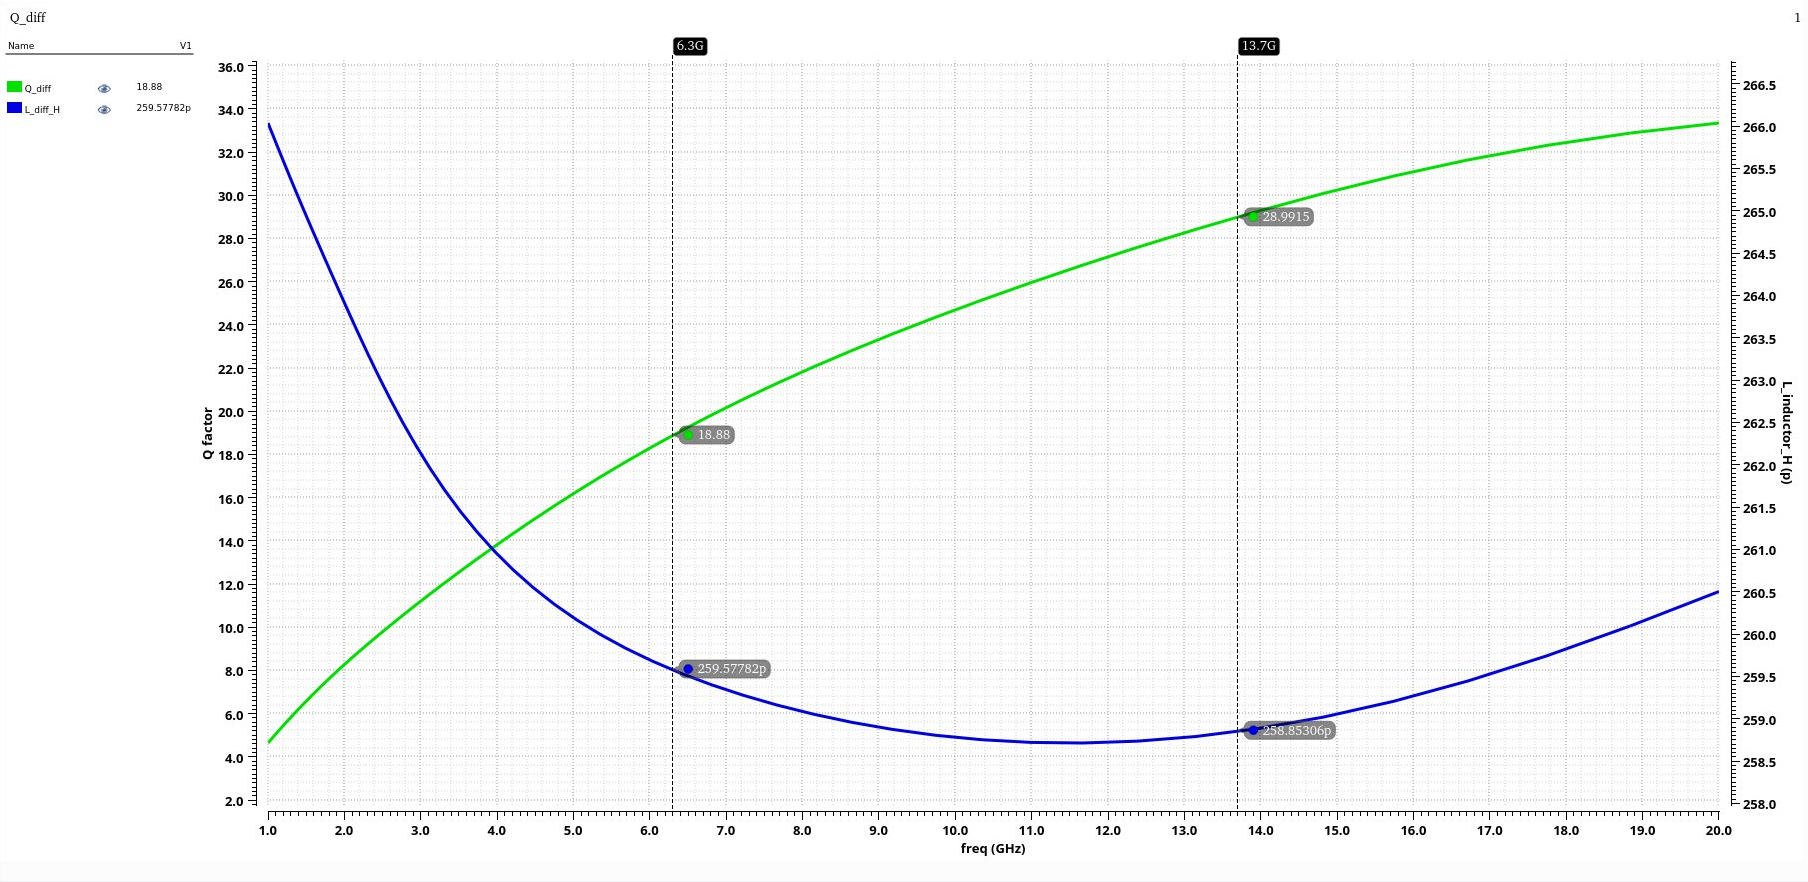
\includegraphics[width=\linewidth]{Figures/QL_inductor.png}
	\caption{Q factor and inductance of L}
	\label{fig:qlinductor}
\end{figure}

Q factor is better at the higher frequency.

Simulated Q factor of both varactors and inductor. Q factor of digital varactor for lower bit controls is not much better than Q of inductor.

Capacitor calculating capacitance and Q factor:

\begin{equation}
	Y_{diff} (im) = imag(ypm('sp 1 1)) + imag(ypm('sp 2 2)) - imag(ypm('sp 2 1)) - imag(ypm('sp 1 2))
\end{equation}

\begin{equation}
	Y_{diff} (re) = real(ypm('sp 1 1)) + real(ypm('sp 2 2)) - real(ypm('sp 2 1)) - real(ypm('sp 1 2))
\end{equation}

Capacitance:
\begin{equation}
	C_{diff} = \dfrac{Y_{diff} (im)}{2\pi f}
\end{equation}

Q factor of capacitor:
\begin{equation}
	Q_C = \dfrac{Y_{diff} (im)}{ Y_{diff} (re)}
\end{equation}

\begin{figure}[h!]
	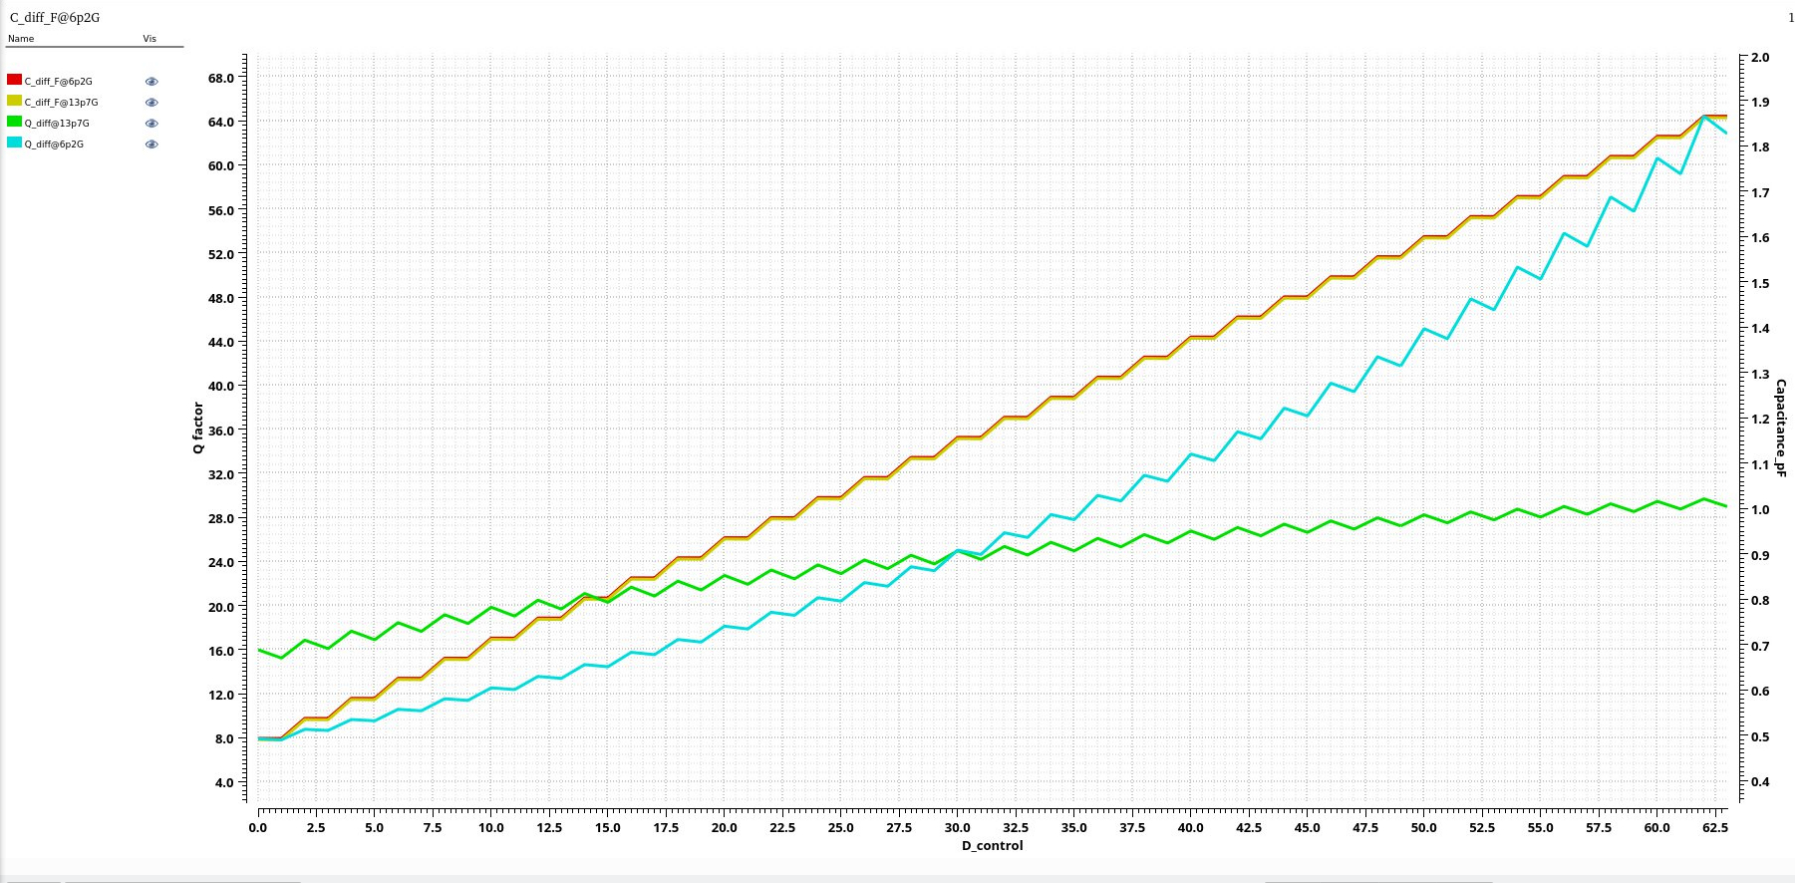
\includegraphics[width=\linewidth]{Figures/Dvaractor.png}
	\caption{C and Q of digital varactor through controls}
	\label{fig:dvaracator}
\end{figure}

More info can be found in  \href{https://ieeexplore.ieee.org/abstract/document/5537949}{\textbf{paper }} A Thorough Analysis of the Tank Quality Factor in LC Oscillators with Switched Capacitor Banks.

How to calculate Q factor of tank from the same paper.

\begin{info}
It can be proved (and it is a well known result) that the quality factor of the tank is equal to the parallel combination of the quality factor of the inductance, $Q_L$, and the quality factor of the capacitance, $Q_C$ , that make up the resonant circuit. Once we have the two quality factors $Q_L$ and $Q_C$ is hence very easy to calculate $Q_T$ .
\end{info}


Found definitions:

\begin{equation}
	Q_{LC} = \dfrac{1}{R}\sqrt{\dfrac{L}{C}} = \frac{f_r}{\Delta f} = \frac{\omega _r}{\Delta \omega} = \dfrac{\tau _d \omega}{2}
\end{equation}

where $\tau _d$ is group delay. Also


\begin{equation}
	Q_{T} = Q_{LC} = \omega \dfrac{ES}{APD}
\end{equation}

where ES is energy stored and APD is average power dissipation.

\begin{question}[\itshape How to calculate group delay using sparam analyis?]
	?
\end{question}

\subsection{Calculating Q factor‚ LC tank by ringing method}

Link to \href{https://www.giangrandi.ch/electronics/ringdownq/ringdownq.shtml}{\textbf{website}} that shows ring down method of calculating Q factor. Not implemented in virtuoso TODO.


%----------------------------------------------------------------------------------------
\section{Figure of Merit different definitions}

\begin{info} % Information block
	The theoretical maxima for the FoM of an oscillator is given by $FoM=174+20log_{10}(Q)$ dBc/Hz
\end{info}

How to calculate oscillator FoM? Is $Q_L$ factor dominant enough to just equate it with LC tank Q facor.

The widely used FOM is calculated by:
\begin{equation}
	FoM = L\{ \Delta \omega \}( \Delta f/f_0)^2 PVCO [mW]
\end{equation}

Where $L\{\Delta \omega\}$ is the phase noise, $ \Delta \frac{f}{f_0}$ is the ratio between the offset frequency and the carrier, and $P_{VCO}$ is the power consumption of the VCO-core. There is also $FoM^T$ and $FoM_A$ 

\begin{equation}
	FoM^T = FoM - 20 \log (\dfrac{FTR}{10})
\end{equation}

and 

\begin{equation}
	FoM_A = FoM + 10 \log (A)
\end{equation}

where A is area [$mm^2$], and FTR frequency tuning range [$\%$]

Information about digital varactor copied from \href{https://www.doe.carleton.ca/~ddchen/Tutorials/DCO.pdf}{\textbf{External link}}

\begin{info} % Information block
Each bit of MIM varactor contains two MIM capacitors connected differentially with a series switch, two pull-up and two pull-down transistors to effectively turn the varactor between its high and low-capacitance states. Measured intrinsic Q of the MIM capacitor is 80 at 3.6 GHz. When is turned on, i.e., high-capacitance state, the varactor Q drops to 30. When is turned off to be in low-capacitance state, the parasitic capacitance of the MIM capacitor and transistors has an effective of 50. The pull-down transistors set the DC levels for drain and source of at 0 V so that
can be efficiently turned into triode region while the weak pull-up transistors set the DC level to VDDOSC to reduce the parasitic capacitance of thus increasing of the parasitic capacitance. The pull-up pMOS can be implemented by either resistors or transistors. The latter was chosen for silicon area efficiency. Compared to MOS varactors, MIM varactors have a much lower . However, since the differential phase-stability inductor is only 10, the impact of lower varactor is tol erable. When the MIM varactor is at its low-capacitance state, the large DCO internal signal swing and the DC level of 1.4-V supply voltage at source/drain of the pull-up transistors force the drain -nwell junction diodes of the pull-up pMOS to momentarily go into forward-bias condition resulting in a latch-up concern. However, since the forward-bias condition occurs only in 50\% of a 3–4 GHz period, the latch-up phenomenon with the parasitic BJTs can not be triggered.
\end{info}

%----------------------------------------------------------------------------------------
\section{Lowering frequency pushing and LDO}

About Frequency pushing from \href{https://www.atlantis-press.com/article/6376.pdf}{\textbf{this paper}}

\begin{info} % Information block
An LC-tank VCO circuit has been implemented in a standard 0.35 $\mu m$ CMOS technology. It is based on a two-transistor biasing structure that improves the performance of frequency pushing and frequency tuning range. Final measurement of proposed structure gives 516 MHz tuning range with 2.278 GHz center frequency and about 0.55$\%$/V frequency pushing in the worst case. The achieved FOM is about -180dBc/Hz, which is very close to the simulated value. This structure is proven to be particularly suitable for achieving low FOM in the VCO circuits having low Q factor LC-tank. Both, the proposed structure and the FOM optimization method, can also be applied to the VCO designs for the applications at higher frequencies, such as 5GHz VCOs for Wireless LAN applications.
\end{info}

\begin{question}[\itshape Can VCO work for lower voltage of 0.9 V?]
	This may be needed if LDO is required because of frequency pushing?
\end{question}

\begin{question}[\itshape Does frequency only happen because of the ripple directly induced by buffers e.g.?]
	Or could it happen because of EM crosstalk?
\end{question}


Is frequency pushing testbench good? Look into this paper. % which paper
Different testbench would be to make a transient change in Vdd and check how much frequency changes.


Results for class C with pmos bias, only dc change of $V_{DD}$:

\begin{center}
	\begin{tabular}{|l|c|c|c|c|c|c|c|c|c|}
		\hline
		Parameter & typical & spec  & min & max & ss -40 & ss 125 & ff -40 & ff 125 & Units \\
		% \hline
		% & \multicolumn{7}{|c|}{VCO Requirements} \\
		\hline
		Frequency Pushing & 43.93 & < 2 &  43.93 & 100.1 & 100.1 & 64.36 & 75.48 & 64.09 & MHz \\ 
		\hline
		Frequency  & 14.6 & > 14.2  & 14.6 & 15.83 & 15.54 & 15.48 & 15.83 & 15.59 & GHz  \\ 
		\hline
	\end{tabular}
\end{center}

This shows some improvement from frequency pushing of 250 - 300 MHz that was observed for the nmos bias of IMEC Scaldio design.

%----------------------------------------------------------------------------------------
\section{Changing topology and lowering phase noise}

Decision on why is single sided oscillator chosen instead of double sided oscillator.

\begin{info}
However, if non-negligible parasitic capacitances are found at the tank outputs, the phase-noise performance of the DS-VCO may be seriously degraded, while that of the SS-VCO remains unaffected.
\end{info}

More on the $\frac{1}{f^2}$ Phase Noise Performance of CMOS Differential-Pair LC-Tank Oscillators in \href{https://backend.orbit.dtu.dk/ws/files/3913656/Andreani.pdf}{\textbf{paper}} by Pietro Andreani.


\subsection{Hybrid class C and class B}

\begin{info}
Further, the proposed VCO solves the issue of the hybrid mixed-signal start-up procedure exposed in [8]. The main drawback of this approach is that, if oscillation stops for some unaccountable reason, the VCO can only be restarted actuating again the whole start-up procedure.
\end{info}

Referenced paper is:

\begin{itemize}
	\item [8] J. Chen, F. Jonsson, M. Carlsson, C. Hedenas, and L.-R. Zheng, “\href{https://ieeexplore.ieee.org/document/5951800}{A low power, startup ensured and constant amplitude class-C VCO in \SI{0.18}{\micro\metre} CMOS},” IEEE Microw. Wireless Compon. Lett., vol. 21, no. 8, pp. 427–429, 2011. Dec. 2008.
\end{itemize}


\subsection{Enhanced Oscillation Swing}

Class-C VCO With Amplitude Feedback Loop for Robust Start-Up and Enhanced Oscillation Swing in \href{https://ieeexplore.ieee.org/stamp/stamp.jsp?arnumber=6377236}{\textbf{this paper.}} Phase noise is lowered by lowering $V_{gbias}$, but it makes oscillations start up harder.

\begin{info}
As noted above, the phase noise improves with increasing the oscillation amplitude, which here would mean lowering the gate bias voltage, $V_{bias}$ . Unfortunately, the original class-C oscillator limits the fixed $V_{bias}$ from being set low enough, otherwise the oscillation may not start up. In [11], a high-swing class-C (HSCC) oscillator was introduced, which removed the tail current transistor of the original class-C oscillator [6]. Instead, an automatic amplitude control was introduced to stabilize the oscillation amplitude. In this work, instead of the transformer used in [11], we choose a simple RC bias circuit.
\end{info}

This is from \href{https://www.semanticscholar.org/paper/Dual-Core-High-Swing-Class-C-VCO-design-Kim-Kim/c9551af0809604f76263af49976df9efc213bb8e}{\textbf{paper}} Dual-Core High-Swing Class-C VCO design, and references 


\begin{itemize}
	\item [6] A. Mazzanti and P. Andreani, “\href{https://ieeexplore.ieee.org/document/4684621}{Class-C harmonic CMOS
	VCOs, with a general result on phase noise},” IEEE J.
	Solid-State Circuits, vol. 43, no. 12, pp. 2716–2729,
	Dec. 2008.
	\item [11] M. Tohidian, A. Fotowat-Ahmadi, M. Kamarei, and F.
	Ndagijimana, “\href{https://ieeexplore.ieee.org/document/6045015}{High-swing class-C VCO},” in Proc.
	ESSCIRC, Sep. 2011, pp. 495–498
\end{itemize}


\subsection{Questions about new double feedback}


Amplitude Control Feedback and Voltage bias control for Robust start up. 

% \begin{question}[\itshape What is?]
% 	This may be needed if LDO is required because of frequency pushing?
% \end{question}


\subsection{OTA1 - Start up  and gate voltage bias control}

Referent voltage should be set and controlled around 800 mV. Need tests for OTAs inside for VCO, currently simulated only PM and DC gain, should test different $V_{ref}$ levels.

\subsection{OTA2 - Start up and bias control}

Referent voltage should be set and controlled around 400 mV. Problem with OTA2 loop is amplifying noise into the tail bias current. So the new problem arises as noise shaping in LOOP2 is needed. If a OTA of low uGBW is used than start up is too slow.


%----------------------------------------------------------------------------------------
\section{Full LO Range and Frequency Recentering}

% TODO Setup the lb vco, and also setup different testbenches for the highest and the lowest frequency available. Add corner analysis PVT.

TODO Add corners for \textbf{fs sf} and similar. Because the LO range is split on two cores, ideally halved. Results are simulated for process and temperature corners: 

\begin{table}[ht]
	\centering
	\begin{tabular}{|l|c|c|c|c|c|}
		\hline
		Core and Specifictaion & min & max & sim(min) & sim(max) & Units \\
		\hline
		\multicolumn{6}{|c|}{VCO core split} \\
		\hline
		High Band Higher limit & 13700 &  & 15580 & 16190  &  MHz  \\ 
		\hline
		High Band Lower limit &  & 10000 & 10870 & 12460 &  MHz  \\ 
		\hline
		High Band range & 3700 &  & 4710 & 3730 &  MHz  \\ 
		\hline
		Low Band Higher limit & 10000 &   & 13230 & 14120 &  MHz  \\ 
		\hline
		Low Band Lower limit &  & 6300 & 6724 & 8028  &  MHz  \\ 
		\hline
		Low Band range & 3700 &  & 6506 & 6092 &  MHz  \\ 
		\hline
	\end{tabular}
	\caption{LO range specification and simulation for Scaldio LC tank}
\end{table}

Expecting the drop for schematic simulated frequency range, covered range should at least be larger than needed when recentered: 

\begin{equation}
	HBFR = 13700 - 10000 = 3700 < 3730 = 16190 - 12460
\end{equation}

For lower band it's similarily calculated

\begin{equation}
	HBFR = 10000 - 6300 = 3700 < 6092 = 14120 - 8028
\end{equation}

Lower and higher band are assymetrical and they overlap for at least:

\begin{equation}
	HBLBoverlap_{high} = 13230 - 10870 = 2360
\end{equation}

\begin{equation}
	HBLBoverlap_{low} = 14120 - 12460 = 1660
\end{equation}

The worst available frequency digital controlled range is $6092 + 3730 - 1660 = 8162$ MHz which is higher than 7400 MHz.

\begin{question}[\itshape Are the two VCO-s in the same process corner at the same time?]
	Yes. If not than the calculations are wrong.
\end{question}

NOTE: Analog varactor 0-Vt-1 change does not work so it wasn't included. Further frequency recentering after extraction will be needed.

%----------------------------------------------------------------------------------------
\section{Pulling testbench and design of VCO buffer}

Needs port at and tuning circuit to keep the reflection at -14 dB. Port of reference impedance 10 k$\Omega$ and portAdapter from rfExamples. S parameter analysis to show if the reflection really is -14 dB? Load impedance increased from 100 fF to 1000 fF. VCO buffer is also needed because of the frequency pulling. Does each core have a buffer or do they share it? first make a buffer than maybe a question.

By adding two buffers from \verb c LO_FDDQ_v6c, \verb c LO_FDDQ_INHB_v5_JCx_scaldio2b  and \verb cLO_FDDQ_BUF_X24 c, frequency pulling drops below 1 MHz. 

So this specification looks fine, testbench shown:


How does portAdapter work?


Frequency pulling mentions coupling (crosstalk) between different blocks on chip and the VCO.
%----------------------------------------------------------------------------------------
\section{Bandgap Voltage}

Bangap voltage source has LN (low noise) control for $V_{bn}$ shown in left of Fig. ~\ref{fig:ac_noise_Bandgap}, for lower voltage reference DAC-s $V_{bp}$ is used without low noise control. Added low noise control at the pmos output is shown on the right side of the Fig ~\ref{fig:ac_noise_Bandgap}. Roll-off frequency of the output noise is determined by the resistence of the native NMOS and loading capacitor. And the lower this frequency is set the larger area or more error is presented to the bandgap voltage. 

\begin{figure}[!ht]
	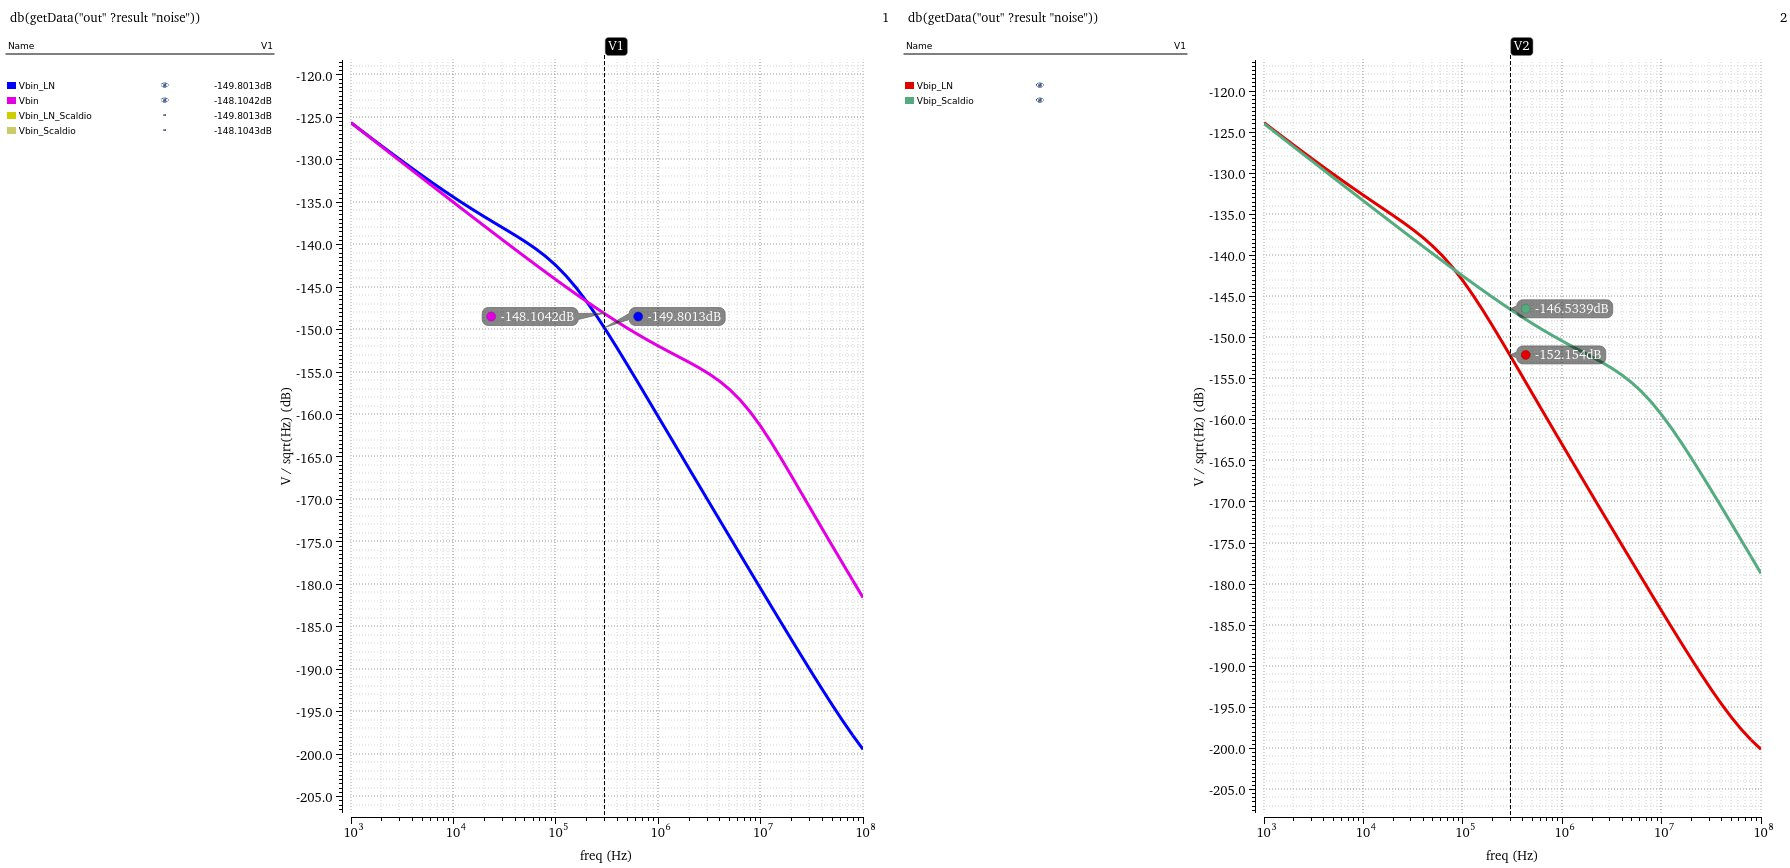
\includegraphics[width=\linewidth]{Figures/ac_noise_Bandgap.jpg}
	\caption{AC Noise of BandGap}
	\label{fig:ac_noise_Bandgap}
\end{figure}


Effect of LN control change is shown as phase noise of pmos biased VCO around 14 GHz. 

\begin{figure}[!ht]
	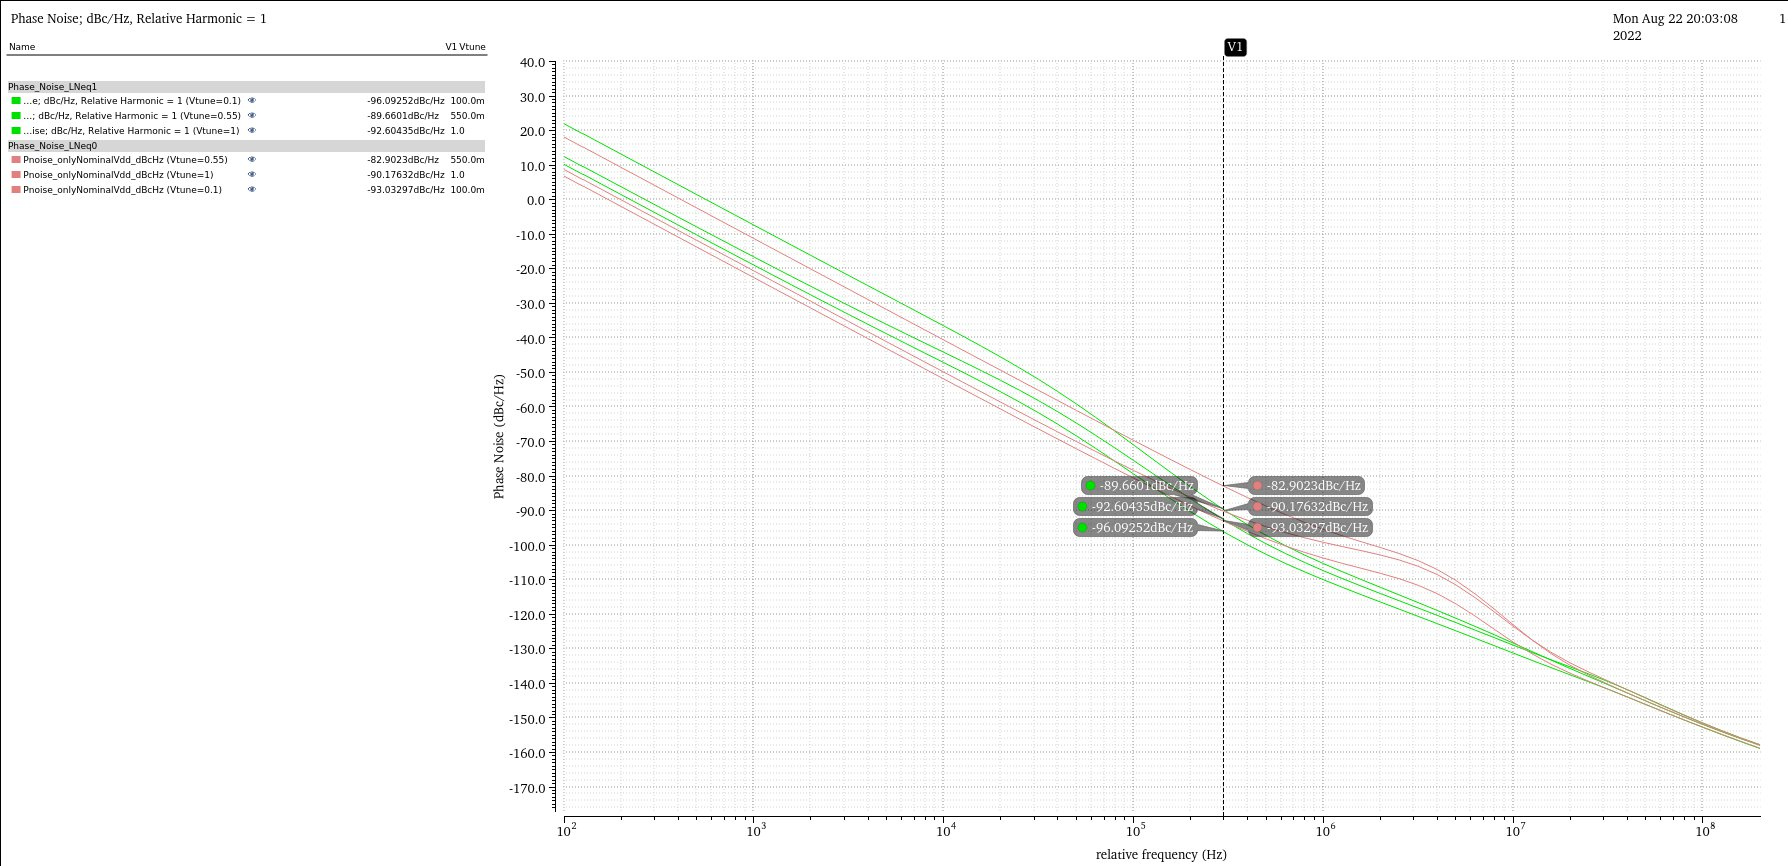
\includegraphics[width=\linewidth]{Figures/phase_noise_Bandgap_pBias_LNeq0&1.jpg}
	\caption{Resulting noise}
	\label{fig:phase_noise_Bandgap_pBias_LNeq0&1}
\end{figure}

TODO Maybe add some results over PVT for Bandgap

TODO Use this info on the original NMOS VCO Scaldio design.

\subsection{PTAT and CTAT, the temperature independant Vbias for cascode}

% \verb c c

TODO Simulate and show results of temperature sweep.


%----------------------------------------------------------------------------------------
\section{Effect of too high tail capacitance}

\begin{figure}[!ht]
	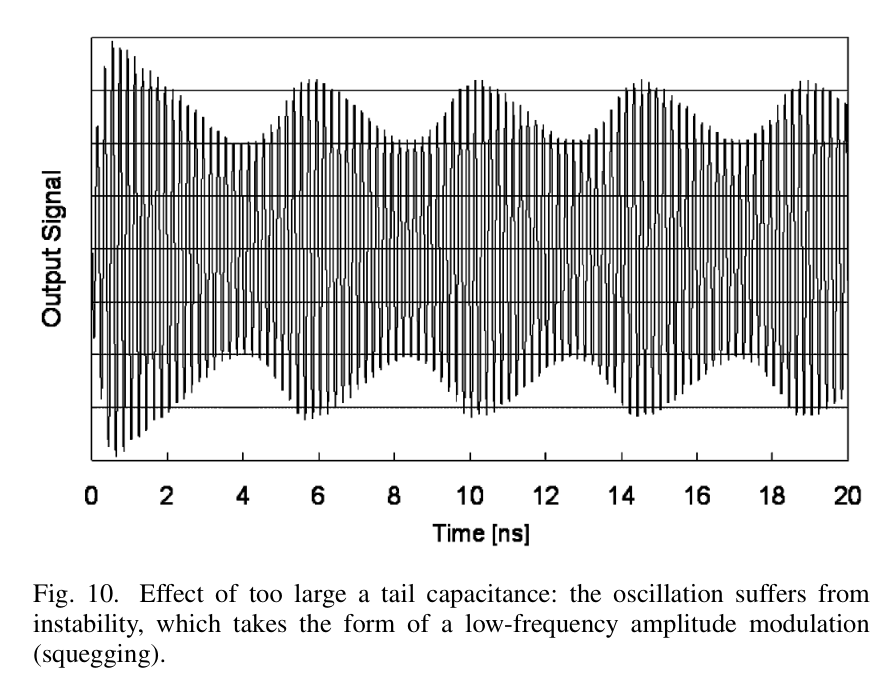
\includegraphics[width=\linewidth]{Figures/squegging.png}
	\caption{Squegging}
	\label{fig:squegging}
\end{figure}

Instability Low frequency amplitude modulation squegging. This was the issue with the original class C with tail current. Is it important for new topology where current bias is PMOS.

TODO simulate for high and for low frequency. How to simulate envelope? 

\section{PLL theory - PLL Lock Detect and calibration}

About PLL Lock Detect:

\begin{info} % Information block
	The ability for a PLL to reliably indicate when it is in lock is critical for many applications. An ideal lock detect circuit gives a high indication when the PLL is locked and a low indication when the PLL is unlocked. When VCO calibration finishes it can be indicative if the lock is detected. 
\end{info}

PLL VCO calibration usually goes as amplitude frequency and then amplitude calibration, or the other way?

Divide and Conquer algorithm


\begin{figure}[!ht]
	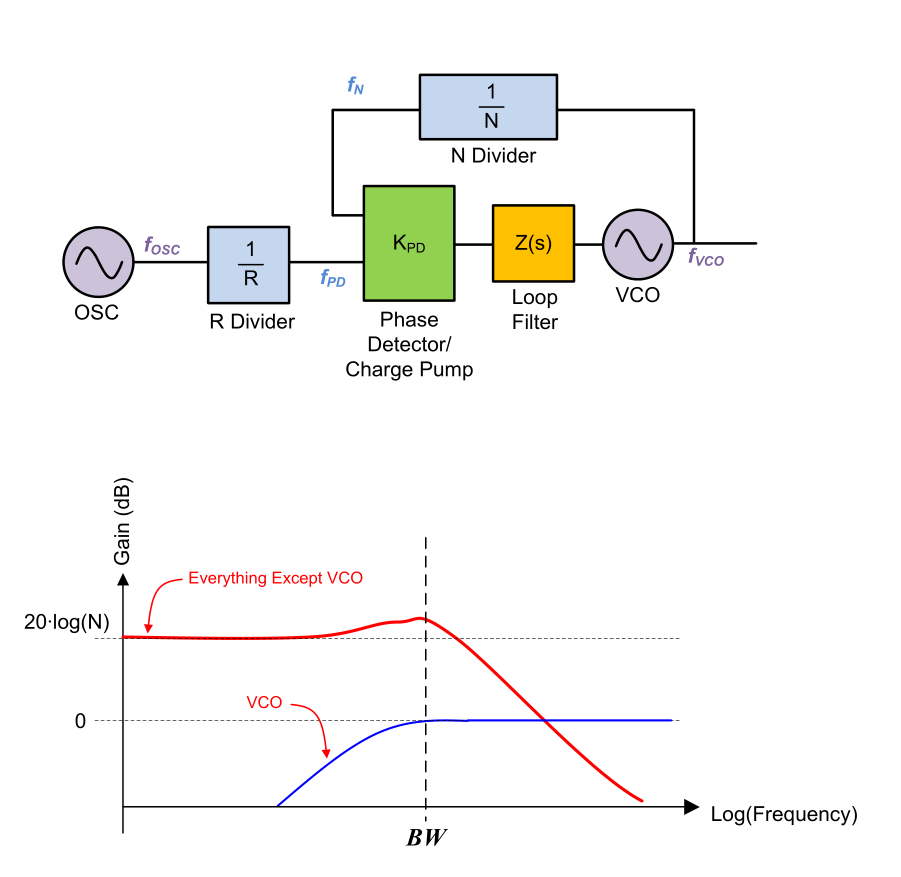
\includegraphics[width=\linewidth]{Figures/PLL_basics_regarding_VCO.png}
	\caption{Gain for VCO and  other blocks inside of PLL}
	\label{fig:PLL_basics_regarding_VCO	}
\end{figure}

\begin{info}
	For the VCO, the noise is suppressed below the loop bandwidth frequency and unshaped above the loop bandwidth.
\end{info}


% 50 or 100 ns for the SAW filter

% differential instead of pseudo differential 

% source degeneration


% \begin{question}[\itshape What kind of output is needed ?]
% 	s
% \end{question}

% Lorem ipsum dolor sit amet, consectetur adipiscing elit. Praesent porttitor arcu luctus, imperdiet urna iaculis, mattis eros. Pellentesque iaculis odio vel nisl ullamcorper, nec faucibus ipsum molestie. Sed dictum nisl non aliquet porttitor. Etiam vulputate arcu dignissim, finibus sem et, viverra nisl. Aenean luctus congue massa, ut laoreet metus ornare in. Nunc fermentum nisi imperdiet lectus tincidunt vestibulum at ac elit. Nulla mattis nisl eu malesuada suscipit.

% % Math equation/formula
% \begin{equation}
% 	I = \int_{a}^{b} f(x) \; \text{d}x.
% \end{equation}

% Aliquam arcu turpis, ultrices sed luctus ac, vehicula id metus. Morbi eu feugiat velit, et tempus augue. Proin ac mattis tortor. Donec tincidunt, ante rhoncus luctus semper, arcu lorem lobortis justo, nec convallis ante quam quis lectus. Aenean tincidunt sodales massa, et hendrerit tellus mattis ac. Sed non pretium nibh. Donec cursus maximus luctus. Vivamus lobortis eros et massa porta porttitor.

% \begin{info} % Information block
% 	This is an interesting piece of information, to which the reader should pay special attention. Fusce varius orci ac magna dapibus porttitor. In tempor leo a neque bibendum sollicitudin. Nulla pretium fermentum nisi, eget sodales magna facilisis eu. Praesent aliquet nulla ut bibendum lacinia. Donec vel mauris vulputate, commodo ligula ut, egestas orci. Suspendisse commodo odio sed hendrerit lobortis. Donec finibus eros erat, vel ornare enim mattis et.
% \end{info}

% %----------------------------------------------------------------------------------------
% %	PROBLEM 1
% %----------------------------------------------------------------------------------------

% \section{Problem title} % Numbered section

% In hac habitasse platea dictumst. Curabitur mattis elit sit amet justo luctus vestibulum. In hac habitasse platea dictumst. Pellentesque lobortis justo enim, a condimentum massa tempor eu. Ut quis nulla a quam pretium eleifend nec eu nisl. Nam cursus porttitor eros, sed luctus ligula convallis quis. Nam convallis, ligula in auctor euismod, ligula mauris fringilla tellus, et egestas mauris odio eget diam. Praesent sodales in ipsum eu dictum.

% %------------------------------------------------

% \subsection{Theoretical viewpoint}

% Maecenas consectetur metus at tellus finibus condimentum. Proin arcu lectus, ultrices non tincidunt et, tincidunt ut quam. Integer luctus posuere est, non maximus ante dignissim quis. Nunc a cursus erat. Curabitur suscipit nibh in tincidunt sagittis. Nam malesuada vestibulum quam id gravida. Proin ut dapibus velit. Vestibulum eget quam quis ipsum semper convallis. Duis consectetur nibh ac diam dignissim, id condimentum enim dictum. Nam aliquet ligula eu magna pellentesque, nec sagittis leo lobortis. Aenean tincidunt dignissim egestas. Morbi efficitur risus ante, id tincidunt odio pulvinar vitae.

% Curabitur tempus hendrerit nulla. Donec faucibus lobortis nibh pharetra sagittis. Sed magna sem, posuere eget sem vitae, finibus consequat libero. Cras aliquet sagittis erat ut semper. Aenean vel enim ipsum. Fusce ut felis at eros sagittis bibendum mollis lobortis libero. Donec laoreet nisl vel risus lacinia elementum non nec lacus. Nullam luctus, nulla volutpat ultricies ultrices, quam massa placerat augue, ut fringilla urna lectus nec nibh. Vestibulum efficitur condimentum orci a semper. Pellentesque ut metus pretium lacus maximus semper. Sed tellus augue, consectetur rhoncus eleifend vel, imperdiet nec turpis. Nulla ligula ante, malesuada quis orci a, ultricies blandit elit.

% % Numbered question, with subquestions in an enumerate environment
% \begin{question}
% 	Quisque ullamcorper placerat ipsum. Cras nibh. Morbi vel justo vitae lacus tincidunt ultrices. Lorem ipsum dolor sit amet, consectetuer adipiscing elit.

% 	% Subquestions numbered with letters
% 	\begin{enumerate}[(a)]
% 		\item Do this.
% 		\item Do that.
% 		\item Do something else.
% 	\end{enumerate}
% \end{question}
	
% %------------------------------------------------

% \subsection{Algorithmic issues}

% In malesuada ullamcorper urna, sed dapibus diam sollicitudin non. Donec elit odio, accumsan ac nisl a, tempor imperdiet eros. Donec porta tortor eu risus consequat, a pharetra tortor tristique. Morbi sit amet laoreet erat. Morbi et luctus diam, quis porta ipsum. Quisque libero dolor, suscipit id facilisis eget, sodales volutpat dolor. Nullam vulputate interdum aliquam. Mauris id convallis erat, ut vehicula neque. Sed auctor nibh et elit fringilla, nec ultricies dui sollicitudin. Vestibulum vestibulum luctus metus venenatis facilisis. Suspendisse iaculis augue at vehicula ornare. Sed vel eros ut velit fermentum porttitor sed sed massa. Fusce venenatis, metus a rutrum sagittis, enim ex maximus velit, id semper nisi velit eu purus.

% \begin{center}
% 	\begin{minipage}{0.5\linewidth} % Adjust the minipage width to accomodate for the length of algorithm lines
% 		\begin{algorithm}[H]
% 			\KwIn{$(a, b)$, two floating-point numbers}  % Algorithm inputs
% 			\KwResult{$(c, d)$, such that $a+b = c + d$} % Algorithm outputs/results
% 			\medskip
% 			\If{$\vert b\vert > \vert a\vert$}{
% 				exchange $a$ and $b$ \;
% 			}
% 			$c \leftarrow a + b$ \;
% 			$z \leftarrow c - a$ \;
% 			$d \leftarrow b - z$ \;
% 			{\bf return} $(c,d)$ \;
% 			\caption{\texttt{FastTwoSum}} % Algorithm name
% 			\label{alg:fastTwoSum}   % optional label to refer to
% 		\end{algorithm}
% 	\end{minipage}
% \end{center}

% Fusce varius orci ac magna dapibus porttitor. In tempor leo a neque bibendum sollicitudin. Nulla pretium fermentum nisi, eget sodales magna facilisis eu. Praesent aliquet nulla ut bibendum lacinia. Donec vel mauris vulputate, commodo ligula ut, egestas orci. Suspendisse commodo odio sed hendrerit lobortis. Donec finibus eros erat, vel ornare enim mattis et.

% % Numbered question, with an optional title
% \begin{question}[\itshape (with optional title)]
% 	In congue risus leo, in gravida enim viverra id. Donec eros mauris, bibendum vel dui at, tempor commodo augue. In vel lobortis lacus. Nam ornare ullamcorper mauris vel molestie. Maecenas vehicula ornare turpis, vitae fringilla orci consectetur vel. Nam pulvinar justo nec neque egestas tristique. Donec ac dolor at libero congue varius sed vitae lectus. Donec et tristique nulla, sit amet scelerisque orci. Maecenas a vestibulum lectus, vitae gravida nulla. Proin eget volutpat orci. Morbi eu aliquet turpis. Vivamus molestie urna quis tempor tristique. Proin hendrerit sem nec tempor sollicitudin.
% \end{question}

% Mauris interdum porttitor fringilla. Proin tincidunt sodales leo at ornare. Donec tempus magna non mauris gravida luctus. Cras vitae arcu vitae mauris eleifend scelerisque. Nam sem sapien, vulputate nec felis eu, blandit convallis risus. Pellentesque sollicitudin venenatis tincidunt. In et ipsum libero. Nullam tempor ligula a massa convallis pellentesque.

% %----------------------------------------------------------------------------------------
% %	PROBLEM 2
% %----------------------------------------------------------------------------------------

% \section{Implementation}

% Proin lobortis efficitur dictum. Pellentesque vitae pharetra eros, quis dignissim magna. Sed tellus leo, semper non vestibulum vel, tincidunt eu mi. Aenean pretium ut velit sed facilisis. Ut placerat urna facilisis dolor suscipit vehicula. Ut ut auctor nunc. Nulla non massa eros. Proin rhoncus arcu odio, eu lobortis metus sollicitudin eu. Duis maximus ex dui, id bibendum diam dignissim id. Aliquam quis lorem lorem. Phasellus sagittis aliquet dolor, vulputate cursus dolor convallis vel. Suspendisse eu tellus feugiat, bibendum lectus quis, fermentum nunc. Nunc euismod condimentum magna nec bibendum. Curabitur elementum nibh eu sem cursus, eu aliquam leo rutrum. Sed bibendum augue sit amet pharetra ullamcorper. Aenean congue sit amet tortor vitae feugiat.

% In congue risus leo, in gravida enim viverra id. Donec eros mauris, bibendum vel dui at, tempor commodo augue. In vel lobortis lacus. Nam ornare ullamcorper mauris vel molestie. Maecenas vehicula ornare turpis, vitae fringilla orci consectetur vel. Nam pulvinar justo nec neque egestas tristique. Donec ac dolor at libero congue varius sed vitae lectus. Donec et tristique nulla, sit amet scelerisque orci. Maecenas a vestibulum lectus, vitae gravida nulla. Proin eget volutpat orci. Morbi eu aliquet turpis. Vivamus molestie urna quis tempor tristique. Proin hendrerit sem nec tempor sollicitudin.

% % File contents
% \begin{file}[hello.py]
% \begin{lstlisting}[language=Python]
% #! /usr/bin/python

% import sys
% sys.stdout.write("Hello World!\n")
% \end{lstlisting}
% \end{file}

% Fusce eleifend porttitor arcu, id accumsan elit pharetra eget. Mauris luctus velit sit amet est sodales rhoncus. Donec cursus suscipit justo, sed tristique ipsum fermentum nec. Ut tortor ex, ullamcorper varius congue in, efficitur a tellus. Vivamus ut rutrum nisi. Phasellus sit amet enim efficitur, aliquam nulla id, lacinia mauris. Quisque viverra libero ac magna maximus efficitur. Interdum et malesuada fames ac ante ipsum primis in faucibus. Vestibulum mollis eros in tellus fermentum, vitae tristique justo finibus. Sed quis vehicula nibh. Etiam nulla justo, pellentesque id sapien at, semper aliquam arcu. Integer at commodo arcu. Quisque dapibus ut lacus eget vulputate.

% % Command-line "screenshot"
% \begin{commandline}
% 	\begin{verbatim}
% 		$ chmod +x hello.py
% 		$ ./hello.py

% 		Hello World!
% 	\end{verbatim}
% \end{commandline}

% Vestibulum sodales orci a nisi interdum tristique. In dictum vehicula dui, eget bibendum purus elementum eu. Pellentesque lobortis mattis mauris, non feugiat dolor vulputate a. Cras porttitor dapibus lacus at pulvinar. Praesent eu nunc et libero porttitor malesuada tempus quis massa. Aenean cursus ipsum a velit ultricies sagittis. Sed non leo ullamcorper, suscipit massa ut, pulvinar erat. Aliquam erat volutpat. Nulla non lacus vitae mi placerat tincidunt et ac diam. Aliquam tincidunt augue sem, ut vestibulum est volutpat eget. Suspendisse potenti. Integer condimentum, risus nec maximus elementum, lacus purus porta arcu, at ultrices diam nisl eget urna. Curabitur sollicitudin diam quis sollicitudin varius. Ut porta erat ornare laoreet euismod. In tincidunt purus dui, nec egestas dui convallis non. In vestibulum ipsum in dictum scelerisque.

% % Warning text, with a custom title
% \begin{warn}[Notice:]
%   In congue risus leo, in gravida enim viverra id. Donec eros mauris, bibendum vel dui at, tempor commodo augue. In vel lobortis lacus. Nam ornare ullamcorper mauris vel molestie. Maecenas vehicula ornare turpis, vitae fringilla orci consectetur vel. Nam pulvinar justo nec neque egestas tristique. Donec ac dolor at libero congue varius sed vitae lectus. Donec et tristique nulla, sit amet scelerisque orci. Maecenas a vestibulum lectus, vitae gravida nulla. Proin eget volutpat orci. Morbi eu aliquet turpis. Vivamus molestie urna quis tempor tristique. Proin hendrerit sem nec tempor sollicitudin.
% \end{warn}

% %----------------------------------------------------------------------------------------

\end{document}
